\section{Quantum Correlations and Entanglement}
  \label{sec:quantum-correlations-and-entanglement}

  \subsection{Non-locality and the Holistic Nature of the Field}
  \label{subsec:non-locality-and-the-holistic-nature-of-the-field}
  In Cosmochrony, quantum entanglement does not arise from nonlocal influences or superluminal signaling.
  Instead, it reflects the persistence of a shared excitation of the $\chi$ field.

  \textit{On the Nature of Quantum Correlations: While this framework might superficially resemble a non-local
  hidden-variable theory, it introduces a critical distinction: the dynamics of the $\chi$ field remains strictly local,
    obeying finite propagation speeds. The correlations emerge from the \textbf{topological connectivity} of the field
    itself. In this sense, entanglement is not an "action at a distance" between two separated entities, but a
    manifestation of a single, extended solitonic configuration. The "hidden variables" are not local properties carried
    by particles, but the global phase and gradient distribution of the underlying $\chi$ field, making the theory
    \textbf{dynamically local but ontologically holist}.}

  When two particles originate from a common interaction or decay process, they correspond to correlated topological
  configurations within the same continuous $\chi$ structure. Although these configurations may later separate
  spatially, they remain parts of a single extended excitation.

  Consider two entangled particles created from a single decay event. Their shared origin imprints a correlated phase
  structure in $\chi$, represented by a single wave packet:
  \begin{equation}
    \chi(x) = \chi_0 \exp\left( -\frac{|x - x_1|^2}{\xi^2} - \frac{|x - x_2|^2}{\xi^2} \right)
  \end{equation}
  where $x_1$ and $x_2$ are their respective positions.
  A measurement or interaction at $x_1$ does not ``send a signal'' to $x_2$; rather, it interacts with a sub-element of
  a globally unified structure.
  This interaction instantaneously constrains the possible outcomes at $x_2$ via the shared $\chi$-configuration, as the
  measurement reveals the state of a single, extended topological object rather than affecting a distant, independent
  one.

  \begin{figure}[h]
    \centering
    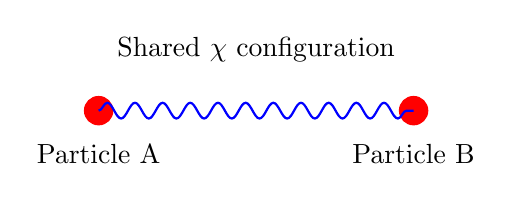
\begin{tikzpicture}[scale=1]

% Particles
      \filldraw[red] (-2,0) circle (0.18);
      \filldraw[red] (2,0) circle (0.18);

      \node[below] at (-2,-0.3) {Particle A};
      \node[below] at (2,-0.3) {Particle B};

% Shared wave
      \draw[blue, thick, decorate, decoration={snake, amplitude=1mm}]
      (-2,0) -- (2,0);

      \node[above] at (0,0.5) {Shared $\chi$ configuration};

    \end{tikzpicture}
    \caption
    {Interpretation of quantum entanglement in Cosmochrony. Entangled particles correspond to persistent shared
    configurations of the $\chi$
      field. Decoherence arises from irreversible fragmentation due to environmental interactions.}
    \label{fig:chi_entanglement}
  \end{figure}

\subsection{Nonlocal Correlations Without Superluminality}\label{subsec:nonlocal-correlations-without-superluminality}

  Because entangled particles are manifestations of the same underlying $\chi$
  excitation, correlations between their measurement outcomes do not require information transfer across space~\cite{bell1964einstein}.
  A measurement performed on one particle locally constrains the global configuration of the shared $\chi$
  excitation.

  This explains the violation of Bell inequalities without invoking superluminal causation.
  Causality is preserved, as no controllable signal propagates between distant measurement events.

  The apparent violation of Bell inequalities arises because the shared $\chi$
  -configuration is established at the time of particle creation, before spatial separation. Measurement
  outcomes are correlated not by superluminal communication, but by sampling the same pre-existing geometric
  structure. This preserves relativistic causality, as no controllable information is transmitted between
  measurement events.

\subsection{Measurement and Decoherence}
    \label{subsec:measurement-and-decoherence}

  Measurement corresponds to a localized interaction that disrupts the coherence of the shared $\chi$ excitation.
  This process effectively partitions the excitation into independent configurations, producing decoherence.

  From this perspective, wavefunction collapse is not a fundamental discontinuity but a dynamical loss of
  topological connectedness within $\chi$ due to environmental interactions.

  \subsubsection{Measurement, Decoherence, and Effective Collapse}
    \label{subsubsec:measurement_clarification}

    In the Cosmochrony framework, the fundamental $\chi$
    field evolves continuously and deterministically at all times. What is conventionally referred to as
    ``wavefunction collapse'' does not correspond to a physical discontinuity of $\chi$
    , but to the breakdown of an effective description in terms of a coherent $\psi$-like excitation.

    A measurement is modeled as a localized interaction between a $\chi$
    -soliton and a macroscopic environment, involving a large number of degrees of freedom. This interaction
    rapidly disperses phase information into the environment, leading to the loss of coherence between different
    fluctuation modes of the $\chi$ field.

    As a result, the initially coherent excitation becomes dynamically partitioned into effectively independent
    configurations, each associated with a distinct, stable outcome. Interference between these configurations
    becomes practically impossible due to the loss of topological connectedness within $\chi$
    across environmental scales.

    Macroscopic superpositions, such as those invoked in Schr\"odinger's cat-type scenarios, are therefore not
    dynamically sustained. The environmental coupling induces rapid decoherence on timescales far shorter than those
    accessible to observation, rendering only a single outcome effectively classical.

    In this sense, measurement corresponds to an emergent, environment-induced selection process rather than a
    fundamental collapse. The apparent definiteness of outcomes arises from the stability and amplification of
    decohered $\chi$ configurations, while the underlying dynamics remains continuous and local.

  Within this framework, measurement does not act on a pre-existing material distribution,
  but on a probabilistic structure shaped by the underlying $\chi$ configuration.
  Orbital probability densities encode stable statistical patterns determined by the topology
  of $\chi$, while individual detection events arise from localized interactions mediated by
  stochastic fluctuations of the field.

  Decoherence corresponds to the disruption of coherent correlations between different
  fluctuation pathways of $\chi$ through environmental coupling.
  This process suppresses interference between alternative manifestations without altering
  the underlying orbital geometry.
  As a result, the stable orbital structure persists at the statistical level, even though
  each measurement event selects a single, contingent outcome.

  In this view, quantum measurement does not collapse a material wave, but localizes a
  fluctuation-induced manifestation within a pre-existing probabilistic pattern imposed by
  the $\chi$ field.

  \subsection{Temporal Ordering and Relativity}\label{subsec:temporal-ordering-and-relativity}

  Because correlations arise from a pre-existing shared structure, their manifestation is independent of the
  temporal ordering of measurements.
  This naturally reconciles entanglement with relativistic causality, as no preferred reference frame is required.

  The apparent instantaneity of entanglement correlations reflects the atemporal connectedness of the $\chi$
  field rather than physical propagation.

\subsection{Limits of Entanglement}
    \label{subsec:limits-of-entanglement}

  Environmental interactions, thermal noise, and coupling to external degrees of freedom progressively disrupt
  shared $\chi$ excitations.
  As a result, entanglement is fragile and degrades with increasing interaction complexity.

  This provides a natural explanation for decoherence timescales observed in quantum systems without introducing
  additional postulates.

\subsection{Summary}
    \label{subsec:summary5}

  Entanglement emerges as the persistence of shared topological excitations within the $\chi$ field.
  Quantum correlations arise without nonlocal signaling, wavefunction collapse, or violations of relativistic
  causality.

  The previous sections described quantum correlations, entanglement, and measurement
  as physical processes occurring within the $\chi$ field itself.
  In the following, we do not introduce new dynamical assumptions,
  but instead examine how the standard quantum-mechanical formalism
  emerges as an effective and approximate description of these underlying processes.
